\chapter{Multi-view recalibration}
\label{cha:multi-view calibration}

\vspace*{-3ex}
The relation between the tools previously defined is provided here, explaining the way they work together in both the acquisition and estimation process.

This chapter is divided in three main sections: \textbf{acquisition}, \textbf{visualization} and \textbf{estimation}. Recall that the goal is to recalibration multiple cameras, using the PR2 as a real example, and focused in the estimation part.

\section{Overview}
\label{sec:estimation_overview}

In Figure \ref{fig:high_level_flow} a high level chart flow is presented: \textbf{1.} camera measurements are collected (checkerboard corners, as explained in section \ref{sec:acquisition}); \textbf{2.} then estimation process is optimizing a non-linear function in order to estimate the cameras poses; \textbf{3.} publishing the result to \texttt{/tf}.

\begin{figure}[!htbp]
 \centering
 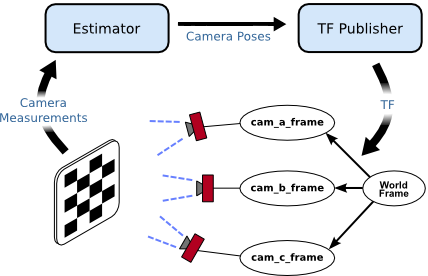
\includegraphics[width=0.5\textwidth]{images/high_level_flow_02.png}
 \caption{High level flow.}
 \label{fig:high_level_flow}
\end{figure}

\noindent
\textbf{Note}: point \textbf{3.} is optional. Since it was desired a visual feedback for the estimation process, it was necessary to considered this option from the beginning in the design. An alternative to \textbf{3.} is to save the result as a new and unique URDF for the particular robot it is being calibrated.



\subsection*{Preliminary: cameras in the PR2}

The PR2 has 6 cameras in its head:
\begin{itemize*}
 \item 2 narrow range. Topics: \texttt{wide\_right\_rect} and \texttt{wide\_left\_rect}.
 \item 2 wide range. Topics: \texttt{narrow\_right\_rect} and \texttt{narrow\_left\_rect}.
 \item 1 Kinect. Topic: \texttt{kinect\_head}.
 \item 1 High definition. Topic: \texttt{Prosilica\_rect}.
\end{itemize*}

\noindent
The initial camera configuration can be seen in Figure \ref{fig:pr2_cameras}, provided by the URDF. \textbf{Note}: this is the initialization and the information to be calibrated.
\begin{figure}[!htbp]
 \centering
 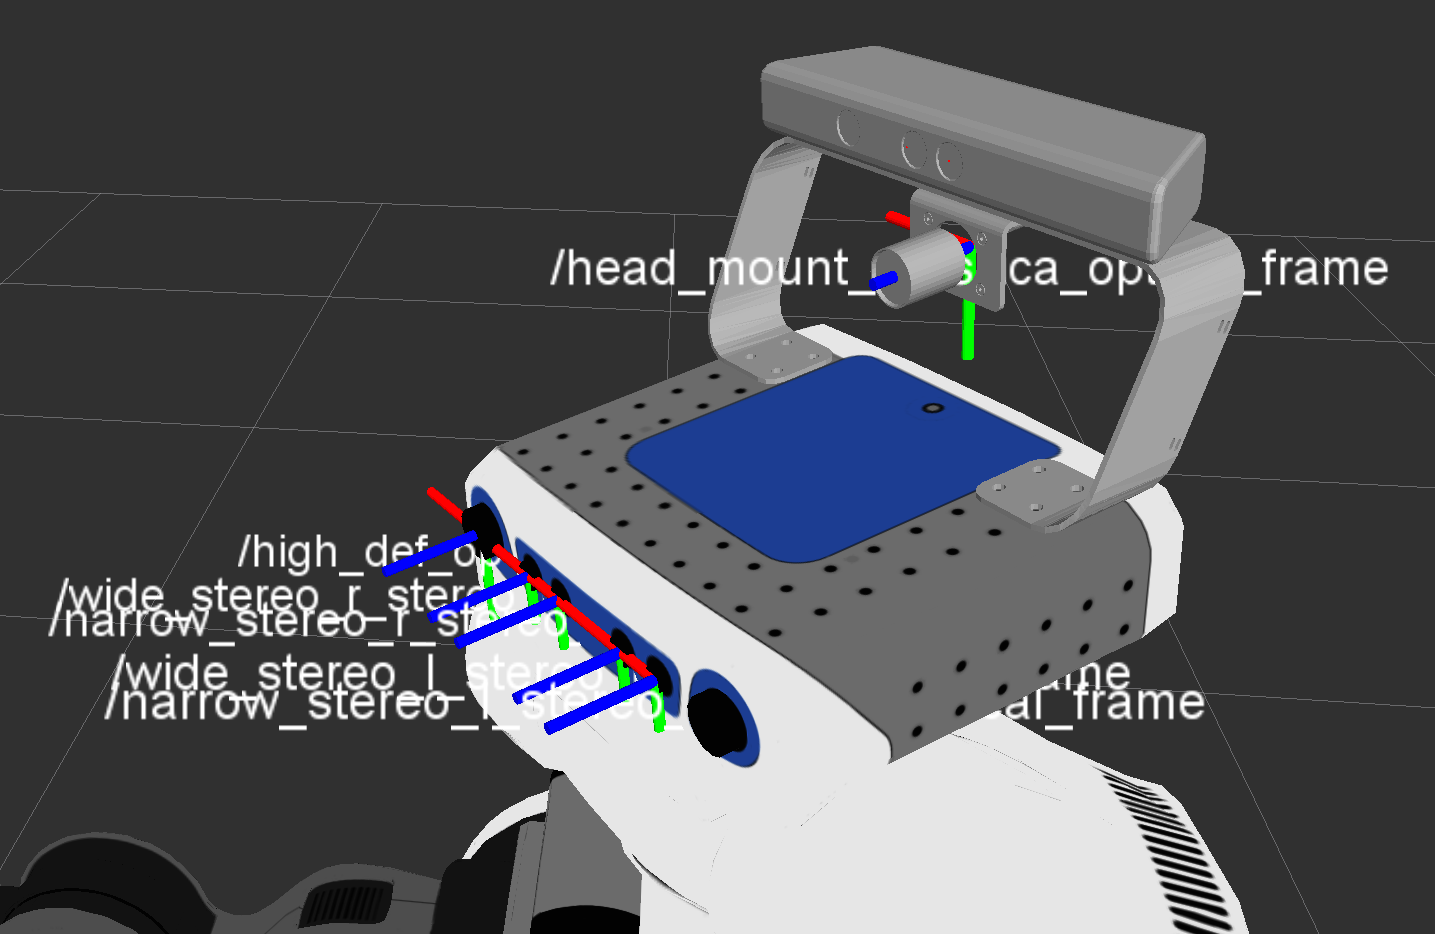
\includegraphics[width=0.55\textwidth]{images/screenshots/PR2_cameras.png}
 \caption{Coordinate system of all the cameras in the PR2 head.}
 \label{fig:pr2_cameras}
\end{figure}






\section{Acquisition process}
\label{sec:acquisition}

This is the \textit{point \textbf{1.}} in the overview (Figure \ref{fig:high_level_flow}). The acquisition part was already implemented, and a full description can be found in the paper  \cite{pr2_calibration_paper} and in the ROS tutorials for the PR2 calibration package.

% The thesis is focused in the estimation part but, in order to reach part, it is necessary first to do some comments regarding the process and
%
% % In the paper  and the ROS tutorials for the PR2 calibration package, the full description of the acquisition process will
% In this section will explain the acquisition process. It will explain


\subsection{Data collection}

In order to sufficiently constrain the non-linear optimization (see \cite{pr2_calibration_paper}), it is needed to collect a large amount of data, and manually collecting this calibration data can be tedious. By having the PR2 hold a checkerboard in its gripper (Figure~\ref{fig:pr2_holdind_cb}), a total of 30 checkerboard poses measurements are collected for each hand. Also, 4 samples of a \textbf{large checkerboard} that is far from the robot in order to help with far-field calibration (see Figure \ref{fig:data_collection01}). This data is saved in a ROS bag (section~\ref{sec:rosbag}) and posteriorly processed for the calibration package.

\noindent

\textbf{Notes}:
\begin{itemize*}
  \item It is important to mention at this point the 2D measurements are obtained from rectified images (section \ref{sec:rectification}). Therefore, working with distortion is happily avoided in the estimation process.
  \item It is assumed all cameras have been intrinsically calibrated in a previous stage.
\end{itemize*}


\begin{figure}[!htbp]
  \centering
  \raisebox{3em}{
    \subfigure
    {
      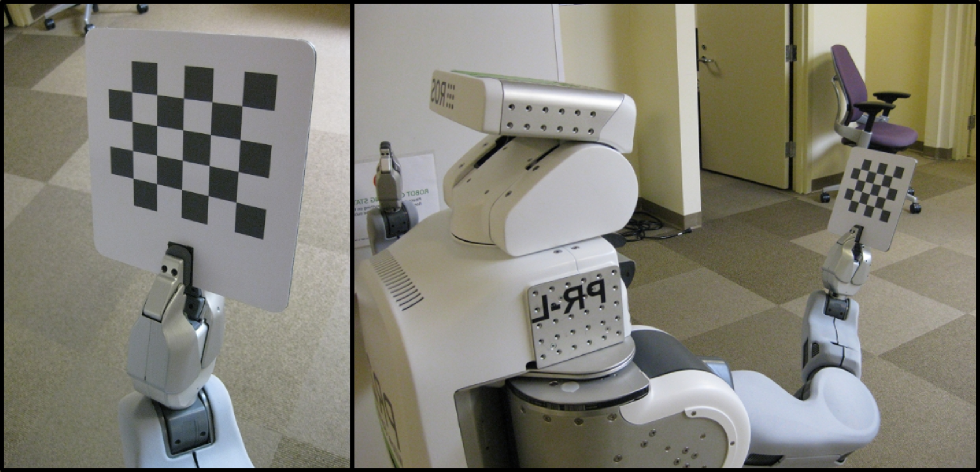
\includegraphics[width=0.5\textwidth]{images/pr2_holdind_cb.png}
    }
  }
  \subfigure
  {
    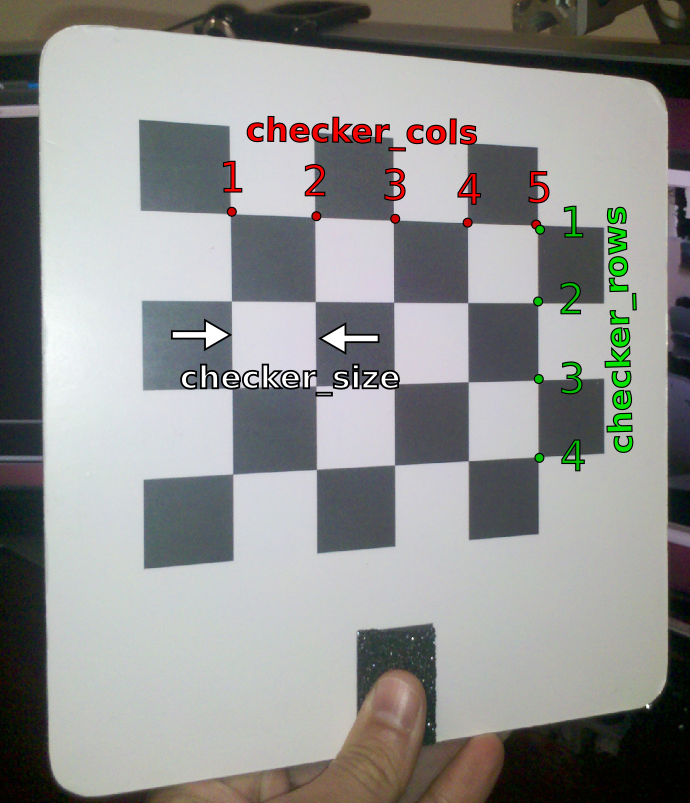
\includegraphics[width=0.35\textwidth]{images/checkerboard01.png}
  }
  \caption{The PR2 holding a checkerboard pattern.}
 \label{fig:pr2_holdind_cb}
\end{figure}


\begin{figure}[!htbp]
 \centering
 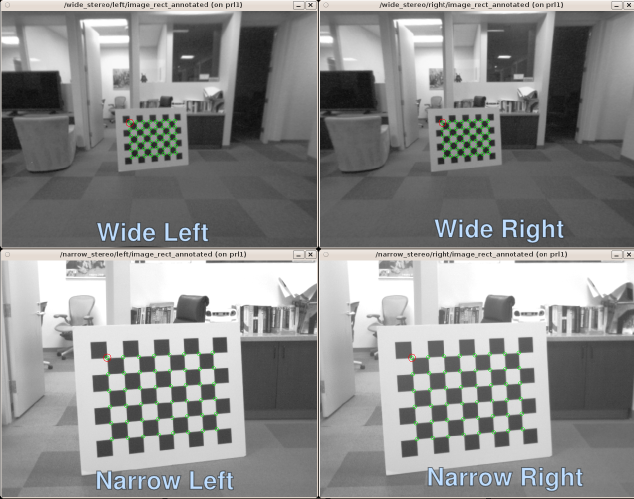
\includegraphics[width=0.7\textwidth]{images/data_collection01.png}
 \caption{Example of \textit{one} sample from 4 different view, using the large checkerboard.}
 \label{fig:data_collection01}
\end{figure}




\subsection{Visualization}

This is the \textit{point \textbf{3.}} in the overview (Figure \ref{fig:high_level_flow}). This part is optional, but it was crucial to understand what was happening and to debug problems and solutions.

Even though publishing to /tf is not difficult to do, it has been time consuming and more details will be given in chapter \ref{cha:implementation}. %, where implementation details are given\footnote{Publish to /tf is mentioned here to be consistent with the overview.}.

For now, let's us concentrate in 3D points visualization, more precisely RViz Markers.

\subsubsection{Visual Markers}

Since checkerboards are seen from multiple views, an idea to check if the system is calibrated is to overlap the 3D obtained from individuals cameras using solvePnP, described in section \ref{sec:solvePnP}.

TODO...


\subsection{Per view optimization}

In order to test the system before going to the global optimization (optimizing the parameters with data in all views), a local optimization per view is performed to see if the process is going in the right path.

TODO... \textit{I want to say I use optimization per view (one checkerboard sample) for testing, before passing to the global optimization (all samples)}



\subsection{Global optimization}

TODO...



\section{Estimation process}
\label{sec:estimation}

TODO...

% Needing to estimate relative poses of several cameras or many poses of a single moving camera is a somewaht common problem. It is often solve by jointly estimating the set of camera poses along with 3D features that are detected by some set of cameras. This approach is called bundle adjustment \cite{BA}.
%
% We have in condition now explain the estimation process, all the needed components have been explained.

% The initial configuration of the cameras is given by the URDF


\subsection{Optimization}

% TODO

% Given the set of many measurements from multiple sensors of multiple views of targets in the world, we want to find the maximum likelihood estimate of cameras poses attached to the a robot head that best explains our measurements. In order to define the residual $r$, it is need to compute the expected measurements to our actual measurements:


TODO....

\subsection{Update robot state}

TODO....



------------------


\subsection{Results}

TODO....

Using solvePnP for points initialization....

Reprojection error first camera...
\begin{figure}[!htbp]
 \centering
 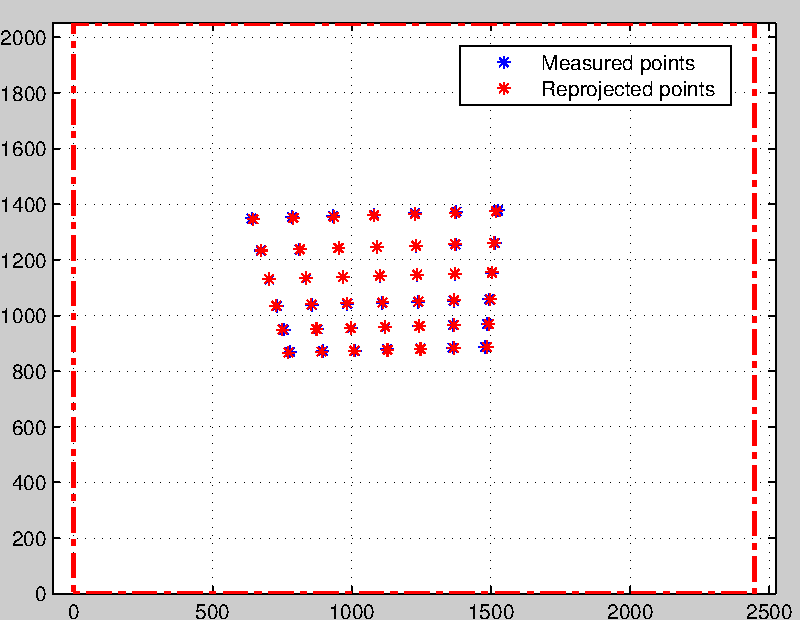
\includegraphics[width=0.5\textwidth]{images/reprojection.pdf}
 \caption{Reprojection error first camera}
 \label{fig:reprojection}
\end{figure}


This solution has a bias...
\begin{figure}[!htbp]
 \centering
 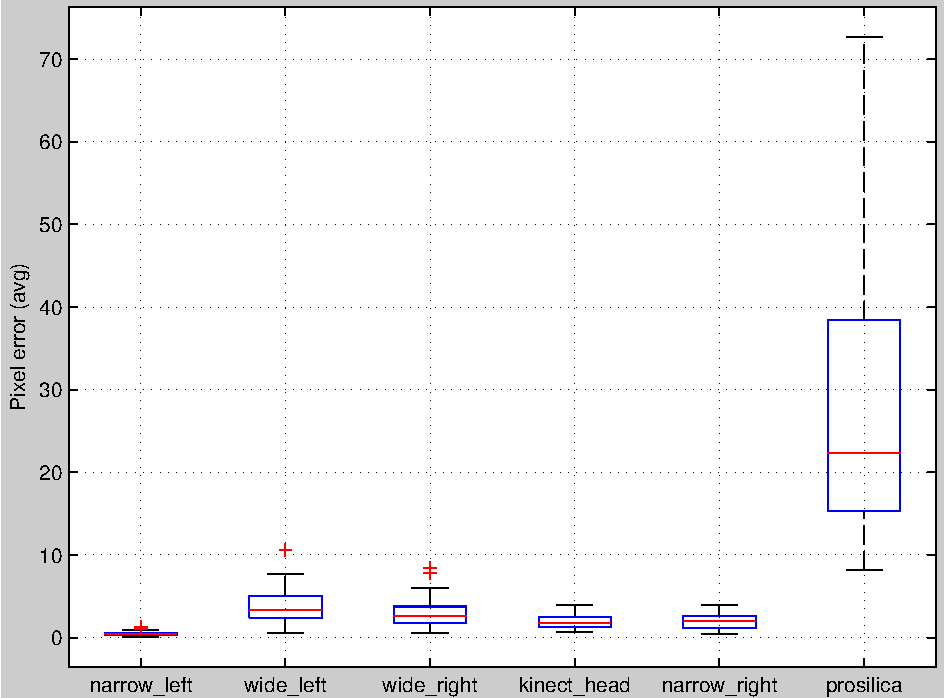
\includegraphics[width=0.5\textwidth]{images/boxplot_stats.pdf}
 \caption{Visible bias in the first camera}
 \label{fig:boxplot_stats}
\end{figure}

Prosilica camera seen to be intrinsically uncalibrated, and it has a lot of errors.
\begin{figure}[!htbp]
 \centering
 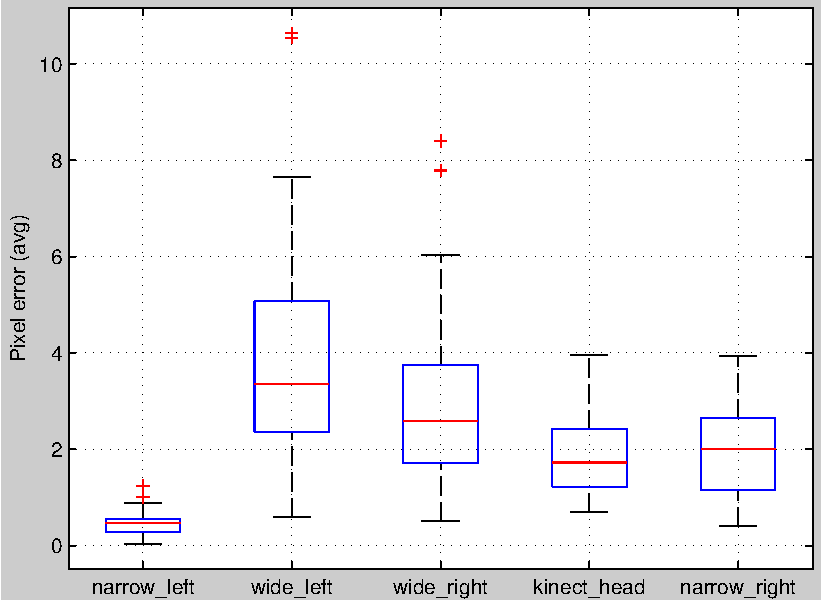
\includegraphics[width=0.5\textwidth]{images/boxplot_stats_without_prosilica.pdf}
 \caption{Boxplot stats without prosilica, bias anyway}
 \label{fig:boxplot_stats_without_prosilica}
\end{figure}


More stats (median, mean, std):
\begin{figure}[!htbp]
 \centering
 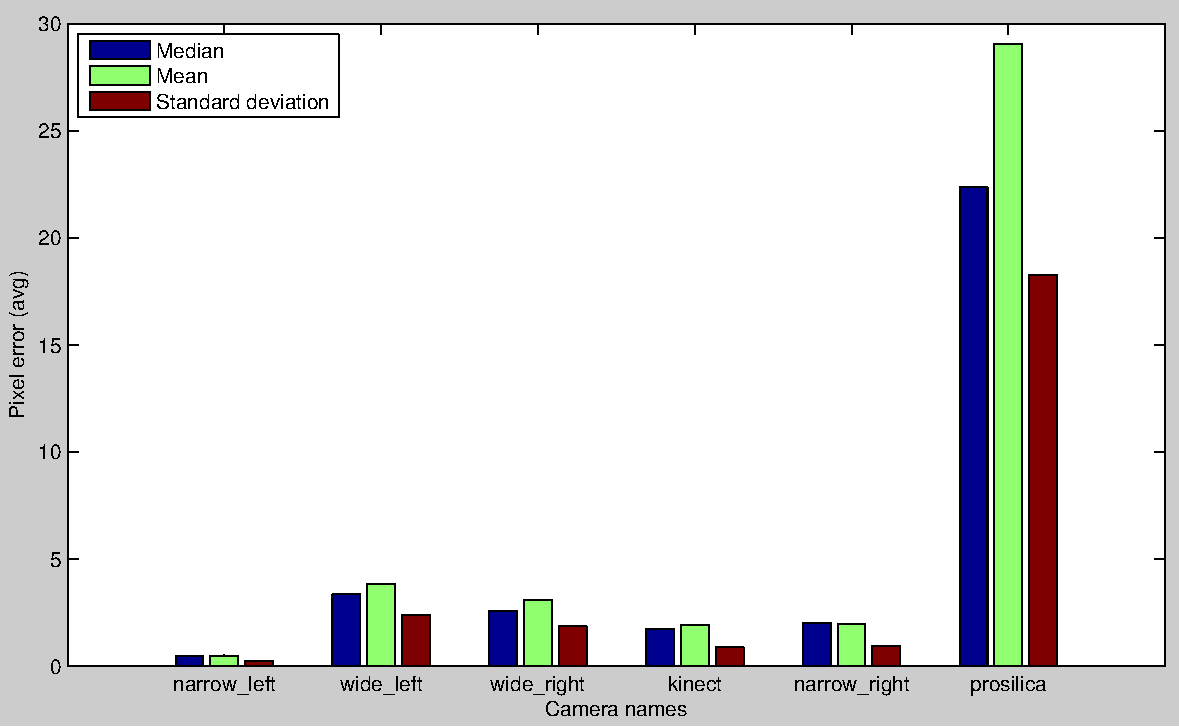
\includegraphics[width=0.5\textwidth]{images/stats.pdf}
 \caption{Median, mean, std}
 \label{fig:stats}
\end{figure}





